\section{Search}


\begin{frame}[fragile]{查找表}

  \begin{center}
    \begin{matrixtable}{1.2cm}{4cm}{1.6cm}{0.6cm}{
        \head{Rank}   & \head{Distribution} & \head{Hits} & \\
        1 & Ubuntu    & 2114 & \down  \\
        2 & Fedora    & 1451 & \up    \\
        3 & Mint      & 1297 & \const \\
        4 & OpenSUSE  & 1228 & \up    \\
        5 & Debian    & 910  & \down  \\ }
    \end{matrixtable} 
  \end{center}

  查找是许多应用系统中最消耗时间的一部分,一个好的查找算法会大大提高运行速度。计
  算机需要存储包含该特定信息的表,才可以高效查找。
\end{frame}


\begin{frame}[fragile]{查找表的分类}
  \begin{easylist} \easyitem
    & 静态查找表
    && 仅作查询和检索操作的查找表。
    & 动态查找表
    && 有时在查询之后,还需要将“查询”结果为“不在查找表中”的数据元素{\em 插入}到查找表中;或者,从查找表中{\em 删除}其“查询”结果为“在查找表中”的数据元素。
  \end{easylist}
\end{frame}


\begin{frame}[fragile]{关键字}
  \begin{easylist} \easyitem
    & 是数据元素(或记录)中某个数据项的值,用以标识(识别)一个数据元素(或记录)。
    & 若此关键字可以识别唯一的一个记录,则称之谓“主关键字”。
    & 若此关键字能识别若干记录,则称之谓“次关键字”。
  \end{easylist}
\end{frame}


\begin{frame}[fragile]{查找}
  \begin{easylist} \easyitem
    & 根据给定的某个值,在查找表中确定一个其关键字等于给定值的数据元素或(记录)  
    & 若查找表中存在这样一个记录,则称“查找成功”:
    && 查找结果:给出整个记录的信息,或指示该记录在查找表中的位置;
    & 否则称“查找不成功”,查找结果:
    && 给出“空记录”或“空指针”。
  \end{easylist}
\end{frame}


\begin{frame}[fragile]{如何进行查找?}
  \begin{easylist} \easyitem
    & 查找的方法取决于查找表的结构。
    & 由于查找表中的数据元素之间不存在明显的组织规律,因此不便于查找。
    & 为了提高查找的效率, 需要在查找表中的元素之间人为地 附加某种确定的关系,换句话说, 用另外一种结构来表示查找表。
  \end{easylist}
\end{frame}


\begin{frame}[fragile]{本章大纲}
  \begin{center}
    \smartdiagram[bubble diagram]{查找表, 1. 静态查找表, 2. 动态查找表, 3. 哈希表}
  \end{center}
\end{frame}

\subsection{1. 静态查找表}
\begin{frame}[plain]
  \frametitle{}
  \centering
  \tikzstyle{mybox} = [draw=blue, fill=green!20, very thick,
  rectangle, rounded corners, inner sep=10pt, inner ysep=20pt]
  \tikzstyle{fancytitle} =[fill=blue, text=white, ellipse]
  
  \vspace{1.0cm}
  \begin{tikzpicture}[transform shape, rotate=0, baseline=-3.5cm]
    \node [mybox] (box) {%
      \begin{minipage}[t!]{0.75\textwidth}
        静态查找:对查找集合只进行查找,不涉及插入和删除操作。或者经过一段时间的查找之后,集中地进行插入和删除等修改操作。

        包括:

        \begin{itemize}
        \item 顺序查找
        \item 折半查找
        \item 分块查找
        \end{itemize}
      \end{minipage}
    };
    \node[fancytitle] at (box.north) {1. 静态查找表};
  \end{tikzpicture}
\end{frame}

\begin{frame}[fragile]
  \frametitle{顺序查找}
  \begin{easylist} \easyitem
    & 又称线性查找,是最基本的查找方法之一

    & 从表的一端向另一端逐个按给定值与关键码进行比较,若找到,查找成功,返回数据元素
    在表中的位置;若未找到与$k$相同的关键码,则返回失败信息。

    & 例:查找 $k=35$
  \end{easylist}
  
  \begin{center}
    \begin{tikzpicture}[box/.style={draw, inner sep=0.2cm, minimum size=1cm}]
      \draw[draw] node[box, fill=blue!20] (b0) {~}
      node[box, right=0 of b0] (b1) {10} 
      node[box, right=0 of b1] (b2) {15}
      node[box, right=0 of b2] (b3) {24}
      node[box, right=0 of b3] (b4) {6}
      node[box, right=0 of b4] (b5) {12}
      node[box, right=0 of b5, fill=red!10] (b6) {35}
      node[box, right=0 of b6] (b7) {40}
      node[box, right=0 of b7] (b8) {98}
      node[box, right=0 of b8] (b9) {55}; 

      \foreach \i in {0,...,9}
      {
        \draw node[above=0 of b\i] (idx_\i) {$\i$};
      };

      \path[] (b9.south) ++(0,-0.8cm) edge[-Latex, dashed] node[right]{$i$} (b9.south);
      \path[] (b6.south) ++(0,-0.8cm) edge[-Latex, very thick, draw=red] node[right]{$i$} (b6.south);

      \path[] (b8.south) ++(0,-1.2cm) edge[-Latex, very thick, draw=blue!60] node[above]{查找方向} ++(-6.5cm,0);
    \end{tikzpicture}
  \end{center}

  注意:下标为0的位置,其哨兵用途。
\end{frame}

\begin{frame}[plain]
  % Define box and box title style
  \tikzstyle{mybox} = [draw=red, fill=blue!20, very thick,
  rectangle, rounded corners, inner sep=10pt, inner ysep=20pt]
  \tikzstyle{fancytitle} =[fill=red, text=white]

  \begin{tikzpicture}
    \node [mybox] (box){%
      \begin{minipage}{0.80\textwidth}
        \begin{itemize}
        \item 分析查找算法的效率,通常用平均查找长度ASL (Average Search Length) 来衡
          量,即在查找成功时所进行的关键码比较次数的期望值。

          顺序查找(等概率情况下):

          \[
            ASL = \sum_{i=1}^{n}\dfrac{1}{n}(n-i+1) = \dfrac{n+1}{2}
          \]

          实际上,数据的查找概率存在相当大的差别!

        \item 在查找概率不同的情况下,应遵循查找表需依据查找概率越高,比较次数越少;查找概率
          越低,比较次数就较多的原则来存储数据元素。
        \end{itemize}
      \end{minipage}
    };
    \node[fancytitle, right=10pt] at (box.north west) {顺序查找的性能分析};
    % \node[fancytitle, rounded corners] at (box.east) {$\clubsuit$};
  \end{tikzpicture}
\end{frame}

\begin{frame}[fragile]
  \frametitle{顺序查找总结}
  \begin{easylist} \easyitem
    & 优点:算法简单而且使用面广。
    
    && 对表中记录的存储没有任何要求,顺序存储和链接存储均可(当然, 链式也只能用顺序
    查找);

    && 对表中记录的有序性也没有要求,无论记录是否按关键码有序均可。

    & 缺点:平均查找长度较大,特别是当待查找集合中元素较多时,查找效率较低。   
  \end{easylist}
\end{frame}

\begin{frame}[fragile]
  \frametitle{(有序表)折半查找}
  \begin{easylist} \easyitem
    & 有序表是表中数据元素按关键码升序或降序排列。

    & 适用于:

    && 线性表中的记录必须按关键码有序;
    
    && 必须采用顺序存储。
  \end{easylist}
\end{frame}

\begin{frame}[fragile]
  \frametitle{请查找14}

  \scalebox{0.7}{
    \begin{tikzpicture}[box/.style={draw, inner sep=0.2cm, minimum size=1cm}]
      \draw[draw] node[box] (b0) {~}
      node[box, right=0 of b0] (b1) {7} 
      node[box, right=0 of b1] (b2) {14}
      node[box, right=0 of b2] (b3) {18}
      node[box, right=0 of b3] (b4) {21}
      node[box, right=0 of b4] (b5) {23}
      node[box, right=0 of b5] (b6) {29}
      node[box, right=0 of b6] (b7) {31}
      node[box, right=0 of b7] (b8) {35}
      node[box, right=0 of b8] (b9) {38}
      node[box, right=0 of b9] (b10) {42}
      node[box, right=0 of b10] (b11) {46}
      node[box, right=0 of b11] (b12) {49}
      node[box, right=0 of b12] (b13) {52} ; 

      \foreach \i in {0,...,13}
      {
        \draw node[above=0 of b\i] (idx_\i) {\i};
      };

      \path[] (b1.south) ++(0,-0.5cm) edge[-Latex, thick] node[below left]{$low=1$} (b1.south);
      \path[] (b13.south) ++(0,-0.5cm) edge[-Latex, thick] node[below right]{$high=13$} (b13.south);
      \path[] (b0.south) ++(-0.5cm,-1cm) edge[draw, dashed] node[above]{\textcircled{1} 设置初始区间} ++(14.5cm,0);


      \path[] (b7.south) ++(0,-1.6cm) edge[-Latex, thick] node[below]{$mid=7$} ++(0,0.5cm)  node[right, xshift=1cm]{\textcircled{2}调整到左半区};

      \path[] (b1.south) ++(0,-2.5cm) edge[-Latex, thick] node[below left]{$low=1$} ++(0,0.5cm);
      \path[] (b6.south) ++(0,-2.5cm) edge[-Latex, thick] node[below right]{$high=6$} ++(0,0.5cm);
      \path[] (b0.south) ++(-0.5cm,-3cm) edge[draw, dashed] node[above]{} ++(14.5cm,0);


      \path[] (b3.south) ++(0,-4cm) edge[-Latex, thick] node[below]{$mid=3$} ++(0,0.5cm)  node[right, xshift=1cm]{\textcircled{3}调整到左半区};

      \path[] (b1.south) ++(0,-4.8cm) edge[-Latex, thick] node[below left]{$low=1$} ++(0,0.5cm);
      \path[] (b2.south) ++(0,-4.8cm) edge[-Latex, thick] node[below right]{$high=2$} ++(0,0.5cm);
      \path[] (b0.south) ++(-0.5cm,-5.2cm) edge[draw, dashed] node[above]{} ++(14.5cm,0);


      \path[] (b1.south) ++(0,-6cm) edge[-Latex, thick] node[below]{$mid=1$} ++(0,0.5cm) node[right, xshift=1cm]{\textcircled{4}调整到右半区};

      \path[] (b2.south) ++(0,-6.8cm) edge[-Latex, thick] node[below left]{$low=2$} ++(0,0.5cm);
      \path[] (b2.south) ++(0,-6.8cm) edge[-Latex, thick] node[below right]{$high=2$} ++(0,0.5cm);
      \path[] (b0.south) ++(-0.5cm,-7.2cm) edge[draw, dashed] node[above]{} ++(14.5cm,0);

      
      \path[] (b2.south) ++(0,-8cm) edge[-Latex, thick] node[below]{$mid=2$} ++(0,0.5cm) node[right, xshift=1cm]{\textcircled{5}查找成功};
    \end{tikzpicture}
  } 
\end{frame}

\begin{frame}[fragile]
  \frametitle{课堂练习:请查找22}
  
  \scalebox{0.7}{
    \begin{tikzpicture}[box/.style={draw, inner sep=0.2cm, minimum size=1cm}]
      \draw[draw] node[box] (b0) {~}
      node[box, right=0 of b0] (b1) {7} 
      node[box, right=0 of b1] (b2) {14}
      node[box, right=0 of b2] (b3) {18}
      node[box, right=0 of b3] (b4) {21}
      node[box, right=0 of b4] (b5) {23}
      node[box, right=0 of b5] (b6) {29}
      node[box, right=0 of b6] (b7) {31}
      node[box, right=0 of b7] (b8) {35}
      node[box, right=0 of b8] (b9) {38}
      node[box, right=0 of b9] (b10) {42}
      node[box, right=0 of b10] (b11) {46}
      node[box, right=0 of b11] (b12) {49}
      node[box, right=0 of b12] (b13) {52} ; 

      \foreach \i in {0,...,13}
      {
        \draw node[above=0 of b\i] (idx_\i) {\i};
      };
    \end{tikzpicture}
  } 
\end{frame}

\begin{frame}[fragile]
  \frametitle{}
  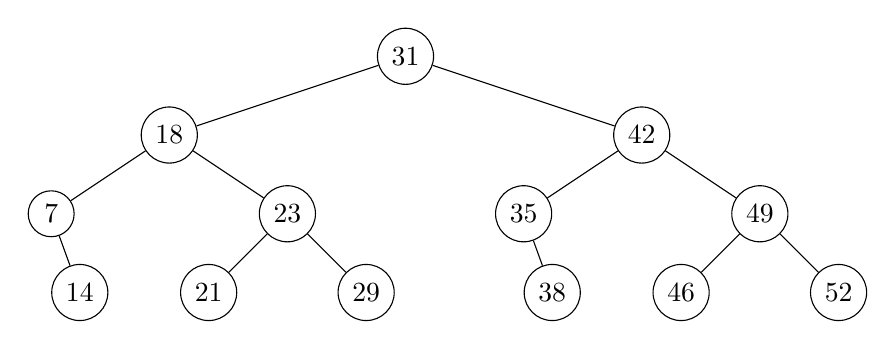
\begin{tikzpicture}[level distance=10mm]
    \tikzstyle{every node}=[draw,circle,inner sep=3pt, minimum size=0.5cm]
    \tikzstyle{level 1}=[sibling distance=60mm,
    set style={{every node}+=[]}]
    \tikzstyle{level 2}=[sibling distance=30mm,
    set style={{every node}+=[]}]
    \tikzstyle{level 3}=[sibling distance=20mm,
    set style={{every node}+=[]}]
    \node {31}
    child {node {18}
      child {node {7}         
        child[right] {node {14}}
      }
      child {node {23}
        child {node {21}}
        child {node {29}}
      }
    }
    child {node {42}
      child {node {35}
        child[right] {node {38}}
      }
      child {node {49}
        child {node {46}}
        child {node {52}}
      }
    };
  \end{tikzpicture}

  从折半查找过程看,以表的中点为比较对象,并以中点将表分割为两个子表,对定位到的子表
  继续这种操作。所以,对表中每个数据元素的查找过程,可用二叉树来描述。
  
  \begin{easylist} \easyitem
    & 折半查找在查找成功时,所进行的关键码比较次数至多为?
    
    & 请问平均查找长度(ASL)是多少?
  \end{easylist}
\end{frame}

\begin{frame}[fragile]
  \frametitle{}

  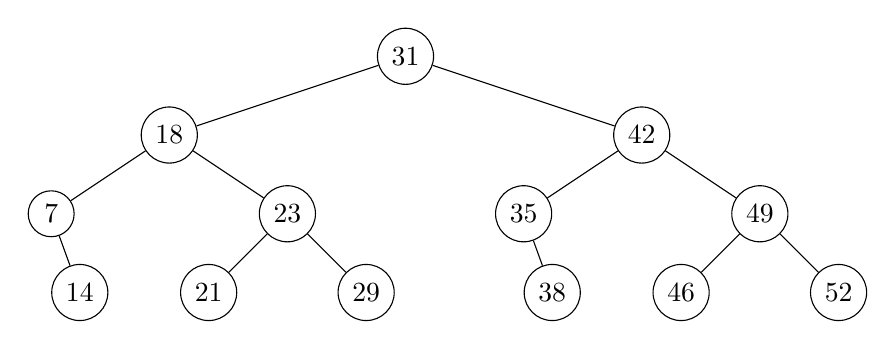
\begin{tikzpicture}[level distance=10mm]
    \tikzstyle{every node}=[draw,circle,inner sep=3pt, minimum size=0.5cm]
    \tikzstyle{level 1}=[sibling distance=60mm,
    set style={{every node}+=[]}]
    \tikzstyle{level 2}=[sibling distance=30mm,
    set style={{every node}+=[]}]
    \tikzstyle{level 3}=[sibling distance=20mm,
    set style={{every node}+=[]}]
    \node {31}
    child {node {18}
      child {node {7}         
        child[right] {node {14}}
      }
      child {node {23}
        child {node {21}}
        child {node {29}}
      }
    }
    child {node {42}
      child {node {35}
        child[right] {node {38}}
      }
      child {node {49}
        child {node {46}}
        child {node {52}}
      }
    };
  \end{tikzpicture}

  \begin{easylist} \easyitem
    & 折半查找在查找成功时,所进行的关键码比较次数至多为?

    \[
      \lfloor log_2 n \rfloor + 1
    \]
    
    & 请问平均查找长度(ASL)是多少?

    \[
      ASL = \dfrac{1}{n}[1 \times 2^0 + 2 \times 2^1 + \cdots + k \times  2^{k-1}]
      \approx \dfrac{n+1}{n} log_2(n+1) - 1
    \]   
  \end{easylist}
\end{frame}


\begin{frame}[fragile]
  \frametitle{分块查找}
  \begin{easylist} \easyitem

    & 分块查找又称索引顺序查找,是对顺序查找的一种改进。适用于表有序或者分块有
    序(后面的子表中所有记录的关键码均大于前一个子表的最大关键码)的情形。

    & 例:对某集合按关键码值31,62,88分为三块建立的查找表及其索引表如下:
  \end{easylist}
  
  \begin{center} 
  \scalebox{0.8}{
    \begin{tikzpicture}[box/.style={draw, minimum size=0.6cm},box2/.style={draw, minimum size=0.7cm, minimum width=1cm, fill=yellow!10}]
      \draw[draw] node[box] (b1) {14} 
      node[box, right=0 of b1] (b2) {31}
      node[box, right=0 of b2] (b3) {8}
      node[box, right=0 of b3] (b4) {22}
      node[box, right=0 of b4] (b5) {18}
      node[box, right=0 of b5] (b6) {43}
      node[box, right=0 of b6] (b7) {62}
      node[box, right=0 of b7] (b8) {49}
      node[box, right=0 of b8] (b9) {35}
      node[box, right=0 of b9] (b10) {52}
      node[box, right=0 of b10] (b11) {88}
      node[box, right=0 of b11] (b12) {78}
      node[box, right=0 of b12] (b13) {70} 
      node[box, right=0 of b13] (b14) {82}
      node[above left=0.2 of b1] {查找表}; 

      \foreach \i in {1,...,14}
      {
        \draw node[below=0 of b\i] (idx_\i) {\i};
      };

      \draw[draw] node[box2, above=1.5cm of b5] (x1) {31} 
      node[box2, right=0 of x1] (x2) {62}
      node[box2, right=0 of x2] (x3) {88}
      node[box2, below=0 of x1] (y1) {1}
      node[box2, below=0 of x2] (y2) {6}
      node[box2, below=0 of x3] (y3) {11}
      node[left=of x1] {索引表}
      node[right=0.2 of x3] {关键码字段}
      node[right=0.2 of y3] {指针字段};

      \path[draw] (y1.center) edge[-Latex] (b1.north) (y2.center) edge[-Latex] (b6.north) (y3.center) edge[-Latex] (b11.north);
    \end{tikzpicture}
  }
\end{center}
 
\end{frame}

\begin{frame}[fragile]
  \frametitle{分块查找}
  \begin{easylist} \easyitem

    & 分块查找要求将查找表分成若干个子表,并对子表建立索引表,查找表的每一个子表由
    索引表中的索引项确定。
    
    & 索引项

    && 关键码字段 (存放对应子表中的最大关键码值) ;
    && 指针字段 (存放指向对应子表的指针) ,并且要求索引项按关键码字段有序。
    
    & 如何根据索引表和查找表进行查找?
  \end{easylist}
  
  \begin{center} 
  \scalebox{0.8}{
    \begin{tikzpicture}[box/.style={draw, minimum size=0.6cm},box2/.style={draw, minimum size=0.7cm, minimum width=1cm, fill=yellow!10}]
      \draw[draw] node[box] (b1) {14} 
      node[box, right=0 of b1] (b2) {31}
      node[box, right=0 of b2] (b3) {8}
      node[box, right=0 of b3] (b4) {22}
      node[box, right=0 of b4] (b5) {18}
      node[box, right=0 of b5] (b6) {43}
      node[box, right=0 of b6] (b7) {62}
      node[box, right=0 of b7] (b8) {49}
      node[box, right=0 of b8] (b9) {35}
      node[box, right=0 of b9] (b10) {52}
      node[box, right=0 of b10] (b11) {88}
      node[box, right=0 of b11] (b12) {78}
      node[box, right=0 of b12] (b13) {70} 
      node[box, right=0 of b13] (b14) {82}
      node[above left=0.2 of b1] {查找表}; 

      \foreach \i in {1,...,14}
      {
        \draw node[below=0 of b\i] (idx_\i) {\i};
      };

      \draw[draw] node[box2, above=1.5cm of b5] (x1) {31} 
      node[box2, right=0 of x1] (x2) {62}
      node[box2, right=0 of x2] (x3) {88}
      node[box2, below=0 of x1] (y1) {1}
      node[box2, below=0 of x2] (y2) {6}
      node[box2, below=0 of x3] (y3) {11}
      node[left=of x1] {索引表}
      node[right=0.2 of x3] {关键码字段}
      node[right=0.2 of y3] {指针字段};

      \path[draw] (y1.center) edge[-Latex] (b1.north) (y2.center) edge[-Latex] (b6.north) (y3.center) edge[-Latex] (b11.north);
    \end{tikzpicture}
  }
\end{center}

\end{frame}

\begin{frame}[fragile]
  \frametitle{分块查找性能分析}

  \begin{easylist}
    & 分块查找含索引表查找和子表查找。
    
    & 设$n$个数据元素的查找表分为$m$个相同大小的子表。则分块查找的平均查找长度为:

    \[
      ASL=\dfrac{m+1}{2} + \dfrac{1}{2} \cdot \dfrac{n}{m+1}
      = \dfrac{m+\dfrac{n}{m}}{2}+1
    \]

    & 可见,平均查找长度和表的总长度$n$、子表个数$m$有关。
  \end{easylist}
  \begin{center} 
  \scalebox{0.8}{
    \begin{tikzpicture}[box/.style={draw, minimum size=0.6cm},box2/.style={draw, minimum size=0.7cm, minimum width=1cm, fill=yellow!10}]
      \draw[draw] node[box] (b1) {14} 
      node[box, right=0 of b1] (b2) {31}
      node[box, right=0 of b2] (b3) {8}
      node[box, right=0 of b3] (b4) {22}
      node[box, right=0 of b4] (b5) {18}
      node[box, right=0 of b5] (b6) {43}
      node[box, right=0 of b6] (b7) {62}
      node[box, right=0 of b7] (b8) {49}
      node[box, right=0 of b8] (b9) {35}
      node[box, right=0 of b9] (b10) {52}
      node[box, right=0 of b10] (b11) {88}
      node[box, right=0 of b11] (b12) {78}
      node[box, right=0 of b12] (b13) {70} 
      node[box, right=0 of b13] (b14) {82}
      node[above left=0.2 of b1] {查找表}; 

      \foreach \i in {1,...,14}
      {
        \draw node[below=0 of b\i] (idx_\i) {\i};
      };

      \draw[draw] node[box2, above=1.5cm of b5] (x1) {31} 
      node[box2, right=0 of x1] (x2) {62}
      node[box2, right=0 of x2] (x3) {88}
      node[box2, below=0 of x1] (y1) {1}
      node[box2, below=0 of x2] (y2) {6}
      node[box2, below=0 of x3] (y3) {11}
      node[left=of x1] {索引表}
      node[right=0.2 of x3] {关键码字段}
      node[right=0.2 of y3] {指针字段};

      \path[draw] (y1.center) edge[-Latex] (b1.north) (y2.center) edge[-Latex] (b6.north) (y3.center) edge[-Latex] (b11.north);
    \end{tikzpicture}
  }
\end{center}

\end{frame}


\subsection{2. 动态查找表}
\begin{frame}[plain]
  \frametitle{}
  \centering
  \tikzstyle{mybox} = [draw=blue, fill=green!20, very thick,
  rectangle, rounded corners, inner sep=10pt, inner ysep=20pt]
  \tikzstyle{fancytitle} =[fill=blue, text=white, ellipse]
  
  \vspace{1.0cm}
  \begin{tikzpicture}[transform shape, rotate=0, baseline=-3.5cm]
    \node [mybox] (box) {%
      \begin{minipage}[t!]{0.75\textwidth}
        动态查找表的特点是,表结构本身是在查找过程中动态生成的,即对于给定的key,若
        表中存在其关键字等于key的记录,则查找成功返回,否则插入关键字等于key的记
        录。

        包括:

        \begin{itemize}
        \item 二叉排序树
        \item 平衡二叉树
        \end{itemize}
      \end{minipage}
    };
    \node[fancytitle] at (box.north) {2. 动态查找表};
  \end{tikzpicture}
\end{frame}

\begin{frame}[fragile]
  \frametitle{二叉排序树}
  \begin{columns}[T] % align columns
    \begin{column}{0.58\linewidth}
      \begin{itemize}
      \item 二叉排序树(Binary Sort Tree)或者是一棵空树;或者是具有下列性质的二叉树:

        \textcircled{1} 若左子树不空,则左子树上所有结点的值均小于根结点的值;若
        右子树不空,则右子树上所有结点的值均大于根结点的值。

        \textcircled{2} 左右子树也都是二叉排序树。

      \item 对二叉排序树进行中序遍历,可以得到一个按关键码有序的序列,因此,一个无序序列
        可通过构造二叉排序树而成为有序序列。
      \end{itemize}
    \end{column}
    \hfill
    \begin{column}{0.38\linewidth}
      \scalebox{0.7}{
        \begin{forest}
          [ 63
          [55
          [42  [10]    [45]  ]
          [58]
          ]
          [90
          [70 [67] [83]]
          [98]
          ]
          ]
        \end{forest}
      }
    \end{column}
  \end{columns}
\end{frame}

\begin{frame}[fragile]
  \frametitle{二叉排序树的查找}

  \begin{columns}[T] % align columns
    \begin{column}{0.58\linewidth}
      \begin{itemize}
      \item 若查找树为空,查找失败;否则将key与查找树的根结点比较

        \textcircled{1} 若相等,查找成功,否则,

        \textcircled{2} 如果key<根结点关键码,继续在以左子树上进行查找

        \textcircled{3} 如果key>根结点关键码,继续在以右子树上进行查找

      \item 例如在右图所示的树上查找45
      \end{itemize}
    \end{column}
    \hfill
    \begin{column}{0.38\linewidth}
      \scalebox{0.7}{
        \begin{forest}
          [ 63
          [55, edge={->, draw=red, thick}
          [42, edge={->, draw=red, thick}  [10]    [45, edge={->, draw=red, thick}]  ]
          [58]
          ]
          [90
          [70 [67] [83]]
          [98]
          ]
          ]
        \end{forest}
      }
    \end{column}
  \end{columns} 
\end{frame}

\begin{frame}[fragile]
  \frametitle{二叉排序树的查找(cont.)}

  \begin{minipage}{0.6\textwidth}
    \begin{easylist}
      & 两树的平均查找长度分别为:

      \[
        ASL_a = \dfrac{1}{6} \times [1+2+2+3+3+3] = \dfrac{14}{6}
      \]
      
      \[
        ASL_b = \dfrac{1}{6} \times [1+2+3+4+5+6] = \dfrac{21}{6}
      \]
      
      & 二叉排序树的平均查找长度和树的形态有关!最好情况是$O(log_2 n)$.
    \end{easylist}
  \end{minipage}%
  \begin{minipage}{0.36\textwidth}
    \scalebox{0.6} {
      \begin{forest}
        [12, grow=-45 [24, grow=-45 [37, grow=-45 [45, grow=-45 [53,grow=-60
        [93]]]]]]         
      \end{forest}
    }
    \scalebox{0.6}{
      \begin{forest}
        [45 [24 [12] [37]] [53,grow=-60 [93]]]
      \end{forest}
    }
  \end{minipage}
\end{frame}

\begin{frame}[fragile]
  \frametitle{二叉排序树的构建 --- 插入节点}
  \begin{minipage}{0.6\textwidth}
    \begin{itemize}
    \item 在查找不成功时,插入该key
      \begin{itemize}
      \item 新插入结点一定是作为叶子结点添加的
      \item 插入位置在查找过程中得到
      \end{itemize}
    \item 例如查找56
    \end{itemize}
  \end{minipage}%
  \begin{minipage}{0.36\textwidth}    
    \scalebox{0.6}{
      \begin{forest}
        [63 [55 [42 [10] [ 45]] [58, grow=245 [56, fill=red!50, dotted]]] [90 [70 [67] [83]] [98]]]
      \end{forest}
    }
  \end{minipage}
\end{frame}

\begin{frame}[fragile]
  \frametitle{序列: 63, 90, 70, 55, 67, 42, 98, 83, 10, 45, 58}
  \small
  \scalebox{0.65}{
    \begin{forest}
      [63]
    \end{forest}\quad
    \begin{forest}
      [63 [, missed] [90, fill=red!10]]
    \end{forest}\quad
    \begin{forest}
      [63 [, missed] [90 [70, fill=red!10] [, missed]]]
    \end{forest}\quad
    \begin{forest}
      [63 [55, fill=red!10] [90 [70] [, missed]]]
    \end{forest}\quad
    \begin{forest}
      [63 [55] [90 [70 [67,fill=red!10] [, missed]] [, missed]]]
    \end{forest}\quad
    \begin{forest}
      [63 [55 [42,fill=red!10] [, missed]] [90 [70 [67] [, missed]] [, missed]]]
    \end{forest}\quad
    \begin{forest} 
      [63 [55 [42] [, missed]] [90 [70 [67] [, missed]] [98, fill=red!10]]]
    \end{forest}
  }

  \scalebox{0.6}{
    
    \begin{forest} 
      [63 [55 [42] [, missed]] [90 [70 [67] [83, fill=red!10]] [98]]]
    \end{forest}
    \quad
    \begin{forest} 
      [63 [55 [42 [10, fill=red!10] [,missed]] [, missed]] [90 [70 [67] [83]] [98]]]
    \end{forest}
    \quad
    \begin{forest} 
      [63 [55 [42 [10] [45, fill=red!10]] [, missed]] [90 [70 [67] [83]] [98]]]
    \end{forest}
    \quad
    \begin{forest} 
      [63 [55 [42 [10] [45]] [58, fill=red!10]] [90 [70 [67] [83]] [98]]]
    \end{forest}
  }
\end{frame}

\begin{frame}[fragile]
  \frametitle{二叉排序树的删除操作}

  依次删除结点45、90,仍要使树保持二叉排序树的特性

  
\end{frame}

\begin{frame}[fragile]{}
  \begin{easylist} \easyitem

  \end{easylist}
\end{frame}


